\chapter{LAMP stack for Kubernetes}
In this chapter the main project is described. First we provide a high-level overview,
followed by a detailed design of the MySQL Operator. We present basic usage examples,
as well as future development ideas. Finally, the main obstacles and design decisions
of the project are explained.

\section{MySQL Operator}

\subsection{High-level overview}
MySQL Operator allows a user to easily deploy replicated MySQL databases on a Kubernetes
cluster. It provides single-command cluster creation, scaling and backup scheduling.
The project is divided into two essential parts:
\begin{itemize}
	\item The actual operator --- a running service which listens for changes on Custom
	Resource objects and creates a new desired configuration on the Kubernetes cluster.
	\item A command line interface --- an optional tool facilitating interaction with
	the created resources.
\end{itemize}

\subsubsection{Functionalities}
The MySQL Operator allows the user to create, delete, update, backup and restore MySQL
clusters.

When \textbf{creating} the cluster, the operator deploys a new instance of a replicated
MySQL database cluster alongside with all additional Kubernetes objects necessary for
a proper deployment. Additionally, rather than initializing a fresh cluster, data may be
\textbf{restored} from a backup file.

When a cluster is to be \textbf{removed}, the operator takes care to delete the cluster
and its configuration from Kubernetes. Unless explicitly specified, database data remains
available, to be cleaned up manually.

A running cluster may be \textbf{updated} by, for example, changing the configuration
(port, password) or scaling the cluster (increasing or decreasing the number of replicas
deployed in the cluster). When such an update is requested, the operator makes sure all
the relevant Kubernetes objects are updated to reflect the new cluster configuration.

\textbf{Scheduling a backup} initiates a recurring backup. The backup job’s behavior is
similar to a cron job’s --- backups are created cyclically at regular intervals.

\subsection{Project Design}

\subsubsection{Custom Resource Definition design}
The main custom resource provided by our project is MySQLCluster. A Custom Resource of
this kind represents a cluster of replicated MySQL servers. It has a unique name specified
by the user and and that name also becomes the name of a Kubernetes Service through which
the database is exposed. Another Custom Resource defined in our project is MySQLBackup.
Objects of this kind are created when the user wants to schedule database backups. Each
instance of this resource corresponds to a backup schedule request for a specific cluster.

\subsubsection{Desing Patterns}
\begin{figure}[!ht]
    \centering
    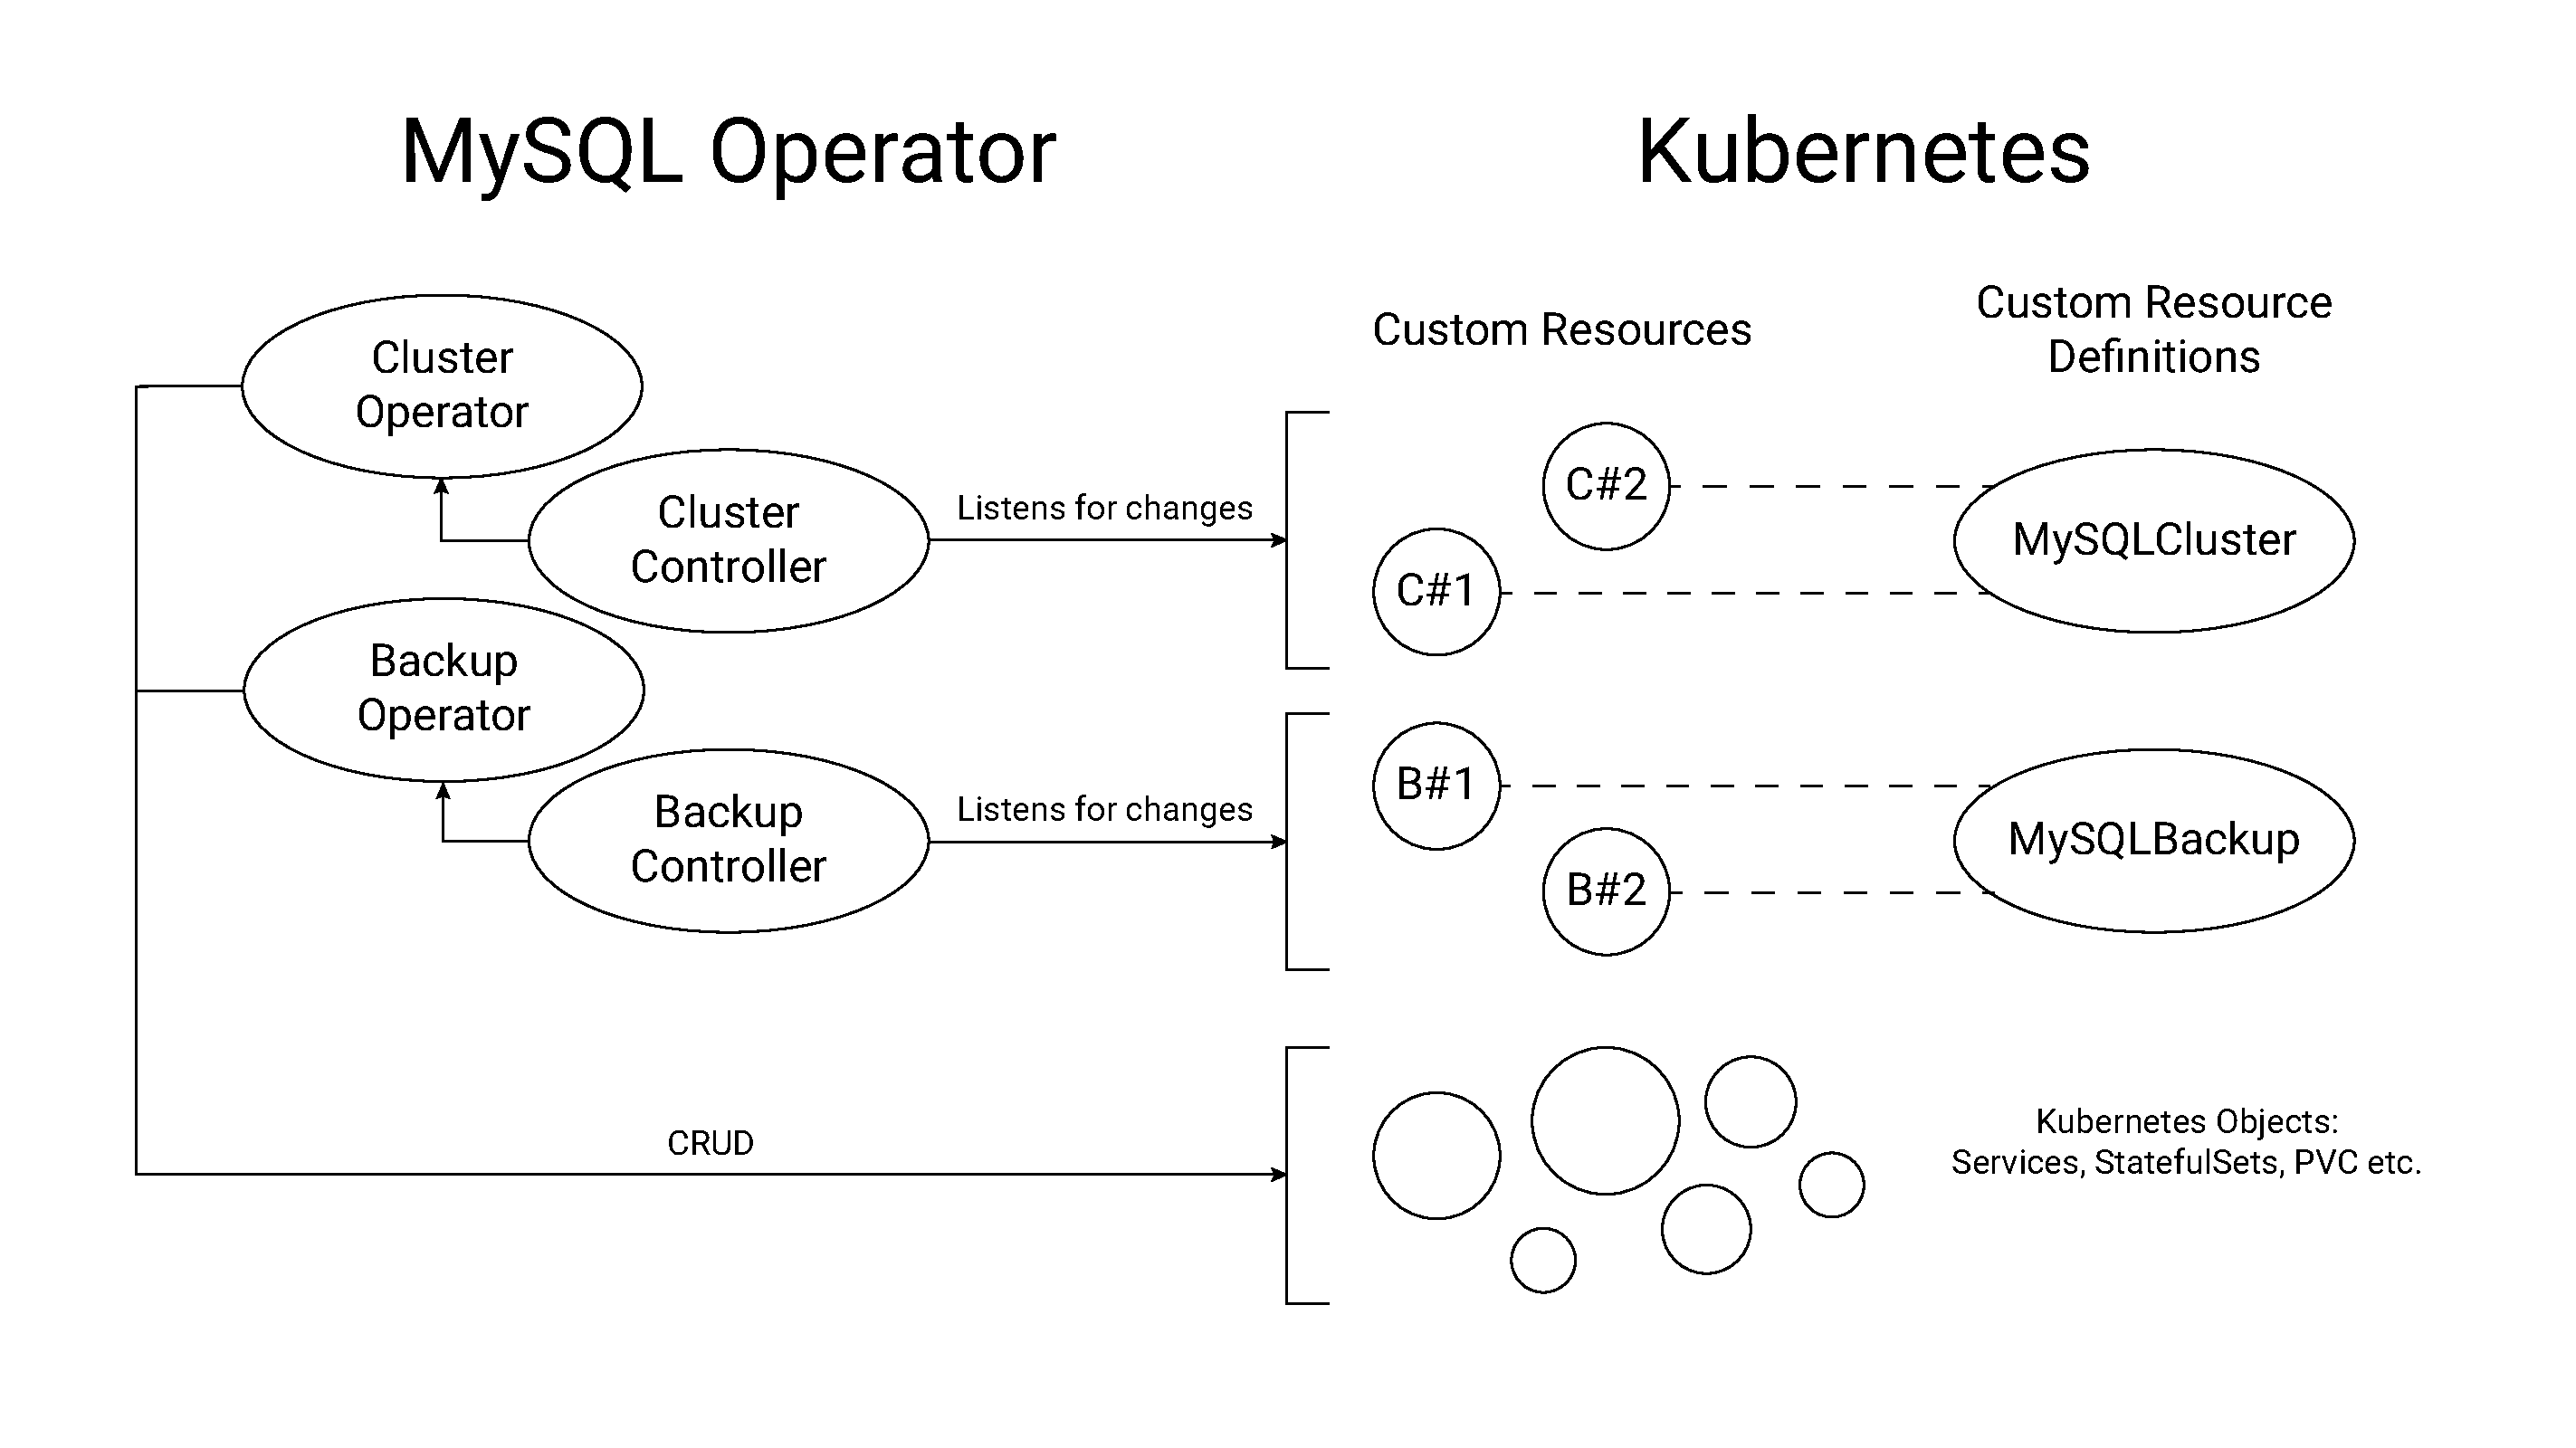
\includegraphics[width=1\textwidth, angle=0]{img/MySQLOperator.pdf}
    \caption{MySQL operator architecture}
\end{figure}

The MySQL Operator’s implementation is primarily based on two common Kubernetes design
patterns: the controller and operator patterns. A \textbf{Controller} is an informer whose
responsibility is to monitor changes in an application’s state. On each change, a predefined
controller function is executed. An \textbf{Operator} builds on ideas from the controller
pattern and basic Kubernetes concepts. It is responsible for creating, configuring and
managing stateful applications running on clusters. Operators extend the Kubernetes API and
create multiple instances of applications like core Kubernetes resources.

We use the controller and operator patterns to manage resources related to both
\texttt{MySQL servers} and \texttt{backup jobs}. Thanks to these constructs we can monitor
Custom Resource instances and adjust all the additional objects accordingly. Both the
databases and backups require a stateful environment, which is exactly the situation for
which the operator pattern was designed for.~\cite{coreos}

\subsection{Detailed design of MySQL cluster}
\subsubsection{Create}
\subsubsection{Services}
\subsubsection{Stateful Set}
\subsubsection{Delete}
\subsubsection{Scale/Update}
\subsubsection{Backup}
\subsubsection{Restore}


\subsection{Command line tool}

\section{Use cases}
In order for the custom resources to be properly processed and an actual MySQL cluster deployed,
a running instance of the MySQL Operator is required inside your Kubernetes infrastructure.

\noindent \texttt{go run operator.go -kubeconfig /path/to/your/kubeconfig}

\subsection{Cluster}

\subsubsection{Create/Restore}
\texttt{kubectl create secret generic my-password --from-literal=password="password" \newline
kubectl apply -f cluster-config.yaml
}

\subsubsection{Data to specify}
\begin{enumerate}
	\item Cluster name\footnote{Cluster name must be unique, it will be the future reference
	to the cluster}
	\item Root password \textit{(Kubernetes secret)}
	\item MySQL port \textit{(optional, defaults to 3306)}
	\item Number of replicas \textit{(optional, default to 1)}
	\item Storage size \textit{(optional, default to 1Gi)}
	\item Custom \textbf{mysql} image \textit{(optional)}
	\item Custom \textbf{xtrabackup} image \textit{(optional)}
	\item Backup name \textit{(optional)}\footnote{If provided, initial cluster data is restored
	from backup}
\end{enumerate}


% \texttt{apiVersion: cr.mysqloperator.grtl.github.com/v1\newline
% kind: MySQLCluster\newline
% metadata:\newline
%   \indent name: "my-cluster"\newline
% spec:\newline
%   \indent name: "my-cluster"\newline
%   \indent password: "my-password"\newline
%   \indent port: 3306\newline
%   \indent storage: "1Gi"\newline
%   \indent mysqlImage: "mysql:latest"\newline
%   \indent xtrabackupImage: "grtl/xtrabackup:latest"\newline
%   \indent restoreFrom:\newline
% 	\indent \indent backupName: "my-backup"\newline
% 	\indent \indent instance: "2017-12-14-01-22"
% }

\subsubsection{Example \textbf{cluster-config.yaml}}
\begin{lstlisting}[caption=cluster-config.yaml,captionpos=b]
apiVersion: cr.mysqloperator.grtl.github.com/v1
kind: MySQLCluster
metadata:
  name: "my-cluster"
spec:
  name: "my-cluster"
  password: "my-password"
  port: 3306
  storage: "1Gi"
  mysqlImage: "mysql:latest"
  xtrabackupImage: "grtl/xtrabackup:latest"
  restoreFrom: 
	backupName: "my-backup"
	instance: "2017-12-14-01-22"
\end{lstlisting}

\subsubsection{Example usage with CLI}
\textbf{Creating new cluster}
\begin{lstlisting}
> cli create cluster "my-cluster" --storage 1Gi
Password: **********<RETURN>
Name: my-cluster
Password: *SECRET*
Port: 3306 [default]
Storage: 1Gi
MySQL Image: mysql:latest [default]
XtraBackup Image: grtl/xtrabackup:latest [default]
Is that correct? [y/N] y<RETURN>
\end{lstlisting}

\noindent \textbf{Restoring cluster from backup}
\begin{lstlisting}
> cli create cluster "my-cluster" --storage 1Gi \
    --from-backup "my-backup:2017-12-14-01-22"
Password: **********<RETURN>
Name: my-cluster
Password: *SECRET*
Port: 3306 [default]
Storage: 1Gi
Restoring from: my-bakcup
MySQL Image: mysql:latest [default]
XtraBackup Image: grtl/xtrabackup:latest [default]
Is that correct? [y/N] y<RETURN>
\end{lstlisting}

\subsubsection{Delete}
\texttt{kubectl delete mysqlcluster my-cluster}

\subsubsection{Data to specify}
\begin{enumerate}
	\item Cluster name
\end{enumerate}

\subsubsection{Example usage with CLI}
\begin{lstlisting}
> cli delete cluster "my-cluster"
Are you sure you want to delete "my-cluster"? [y/N] y<RETURN>
\end{lstlisting}

\subsubsection{Update}
\texttt{kubectl apply -f cluster-config.yaml}

\subsubsection{Data to specify}
\begin{enumerate}
	\item Cluster name
	\item Root password \textit{(Kubernetes secret)}
	\item MySQL port \textit{(optional, defaults to 3306)}
	\item Number of replicas \textit{(optional, default to 1)}
\end{enumerate}

\subsubsection{Example usage with CLI}
\begin{lstlisting}
> cli update cluster "my-cluster" --replicas=4
Cluster: my-cluster
Replicas: 2 -> 4
Is that correct? [y/N] y<RETURN>
\end{lstlisting}

\subsection{Backup}

\subsubsection{Create}
\texttt{kubectl create -f backup-config.yaml}

\subsubsection{Data to specify}
\begin{enumerate}
	\item Backup name \textit{(optional: defaults to auto generated based on cluster name)}
	\item Cluster name
	\item Time \textit{(CRON style)}
\end{enumerate}

\subsubsection{Additional info}
Database will be backed up in an automatically claimed Persistent Volume with the size
calculated based on the cluster current database size.

\subsubsection{Example \textbf{backup-config.yaml}}
\begin{lstlisting}[caption=backup-config.yaml,captionpos=b]
apiVersion: cr.mysqlbackup.grtl.github.com/v1
kind: MySQLBackup
metadata:
  name: "my-backup"
spec:
  cluster: "my-cluster"
  time: "*/1 * * * *"
\end{lstlisting}

\subsubsection{Example usage with CLI}
\begin{lstlisting}
> cli create backup "my-backup" --cluster "my-cluster"
Password: **********<RETURN>
Backup: my-backup
Cluster: my-cluster
Is that correct? [y/N] y<RETURN>
\end{lstlisting}

\section{Obstacles}

\section{Future development}
